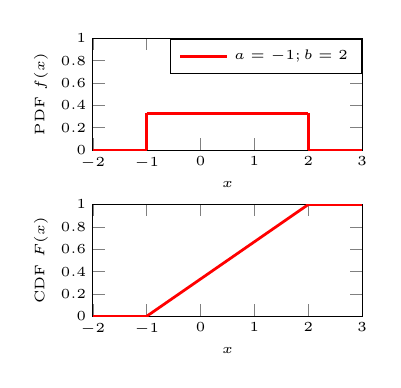
\begin{tikzpicture}
    \tiny
    \begin{axis}[
            width = 5cm,
            height = 3cm,
            % width = \linewidth,
            % unit vector ratio={1 1},
            name = axis1,
            xmin = -2,
            ymin  = 0,
            xmax = 3,
            ymax = 1,
            xtick distance=1,
            % ytick={0,3,8},
            % yticklabels={0,$\lambda_1$,$\lambda_2$},
            % xtick = {0},
            % xticklabel=\empty,
            xlabel={$x$},
            ylabel={PDF $f(x)$},
            legend style={at={(1,1)},anchor=north east},
            legend style={font=\tiny},
            grid style=dashed,
        ]
        \addplot [
            color=red,
            line width = 1pt]
        coordinates {
                (-2,0)
                (-1,0)
            };
        \addplot [
            color=red,
            line width = 1pt]
        coordinates {
                (-1,0)
                (-1,0.33)
            };
        \addplot [
            color=red,
            line width = 1pt]
        coordinates {
                (-1,0.33)
                (2, 0.33)
            };
        \addplot [
            color=red,
            line width = 1pt]
        coordinates {
                (2, 0.33)
                (2, 0)
            };
        \addplot [
            color=red,
            line width = 1pt]
        coordinates {
                (2, 0)
                (3, 0)
            };
        \addlegendentry{$a = -1; b = 2$}
    \end{axis}
    \begin{axis}[
            width = 5cm,
            height = 3cm,
            % width = \linewidth,
            % unit vector ratio={1 1},
            name = axis2,
            xmin = -2,
            ymin  = 0,
            xmax = 3,
            ymax = 1,
            xtick distance=1,
            % ytick={0,3,8},
            % yticklabels={0,$\lambda_1$,$\lambda_2$},
            % xtick = {0},
            % xticklabel=\empty,
            at=(axis1.below south west), anchor=above north west,
            xlabel={$x$},
            ylabel={CDF $F(x)$},
            legend style={at={(1,0)},anchor=south east},
            legend style={font=\tiny},
            grid style=dashed,
        ]
        \addplot [
            color=red,
            line width = 1pt]
        coordinates {
                (-2,0)
                (-1,0)
            };
        \addplot [
            color=red,
            line width = 1pt]
        coordinates {
                (-1,0)
                (2,1)
            };
        \addplot [
            color=red,
            line width = 1pt]
        coordinates {
                (2, 1)
                (3, 1)
            };
    \end{axis}
\end{tikzpicture}